\documentclass{article}
\usepackage{ctex}
\usepackage{graphicx}
\usepackage{amsmath}
\usepackage{esint}%环路重积分用
\usepackage{indentfirst}
\usepackage{titlesec}
\usepackage{setspace}
\usepackage{subfigure}
\usepackage{caption}
\usepackage{float}
\usepackage{booktabs}
\usepackage{geometry}
\usepackage{multirow}
\usepackage{hyperref}

\hypersetup{
	colorlinks=true,
	linkcolor=blue,
	filecolor=magenta,      
	urlcolor=cyan,
	pdftitle={Overleaf Example},
	pdfpagemode=FullScreen,
}
\geometry{left=1.2cm,right=1.2cm,top=2cm,bottom=2cm}
\title{\songti \zihao{2}\bfseries 闪锌矿晶体的讨论}
\titleformat*{\section}{\songti\zihao{4}\bfseries}
\titleformat*{\subsection}{\songti\zihao{5}\bfseries}
\renewcommand\thesection{\arabic{section}}
\author{王启骅 PB20020580}
\begin{document}
	\maketitle
		\section{结构}
	闪锌矿$ (ZnS) $结构如图1所示,S原子(绿色)位于$ 000,0\frac{1}{2}\frac{1}{2},\frac{1}{2}0\frac{1}{2},\frac{1}{2}\frac{1}{2}0 $,Zn原子(紫色)坐标$ \frac{1}{4}\frac{1}{4}\frac{1}{4},\frac{1}{4}\frac{3}{4}\frac{3}{4},\frac{3}{4}\frac{1}{4}\frac{3}{4},\frac{3}{4}\frac{3}{4}\frac{1}{4} $
	\begin{figure}[!h]
		
		\centering
		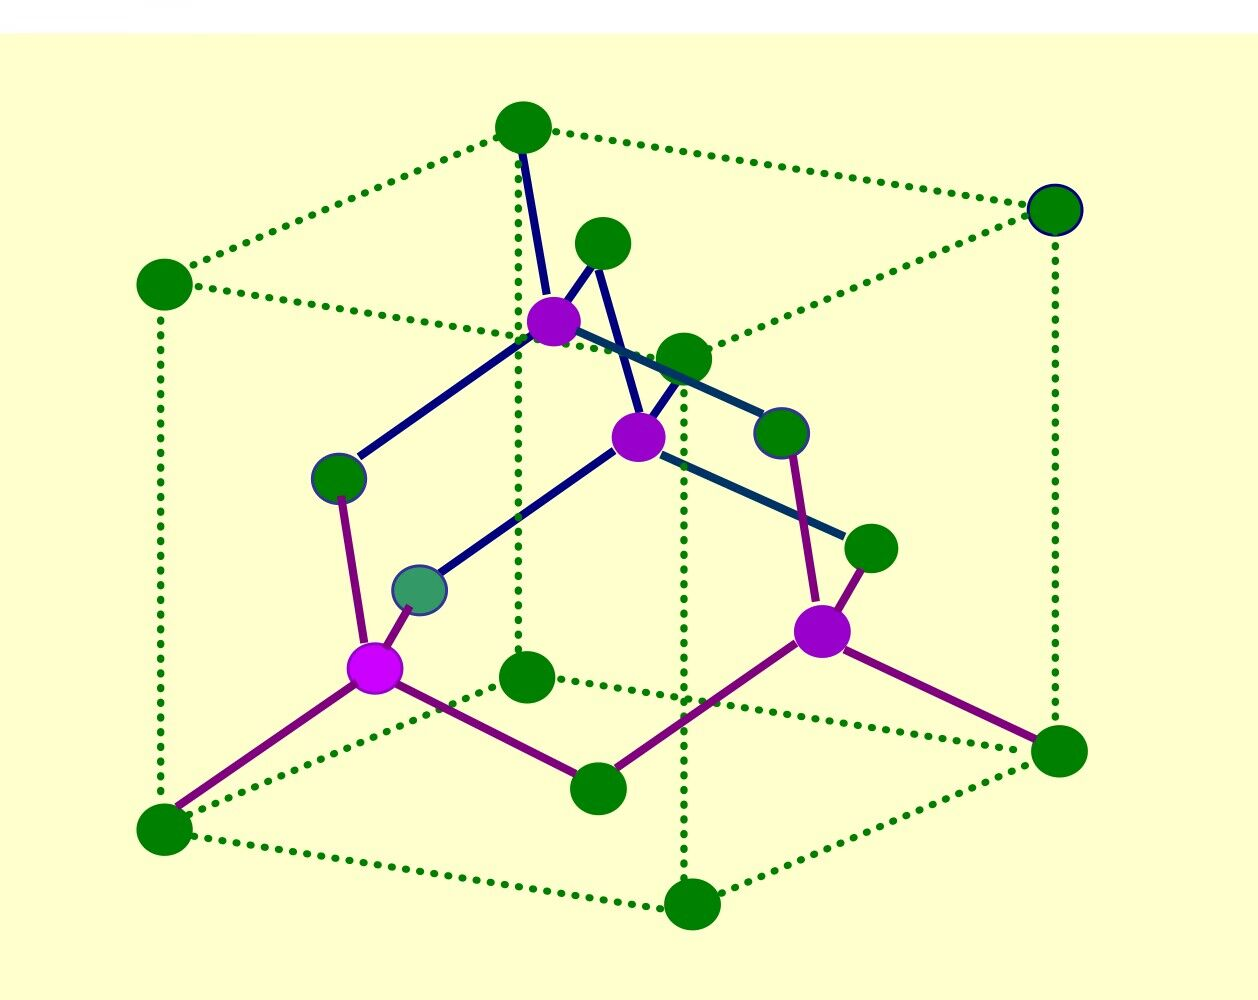
\includegraphics[scale=0.2]{结构}
		\captionsetup{font={small},labelfont=bf}
		\caption{\heiti\zihao{-5}闪锌矿结构}
		
	\end{figure}
	
	
	可以取如图2一个S原子连接四个Zn原子(由每个Zn与4个S相连,各占有$  \frac{1}{4} $)为一个基元,则可以等效于面心立方点阵。
	\begin{figure}[!h]
		\centering
		\subfigure[基元]{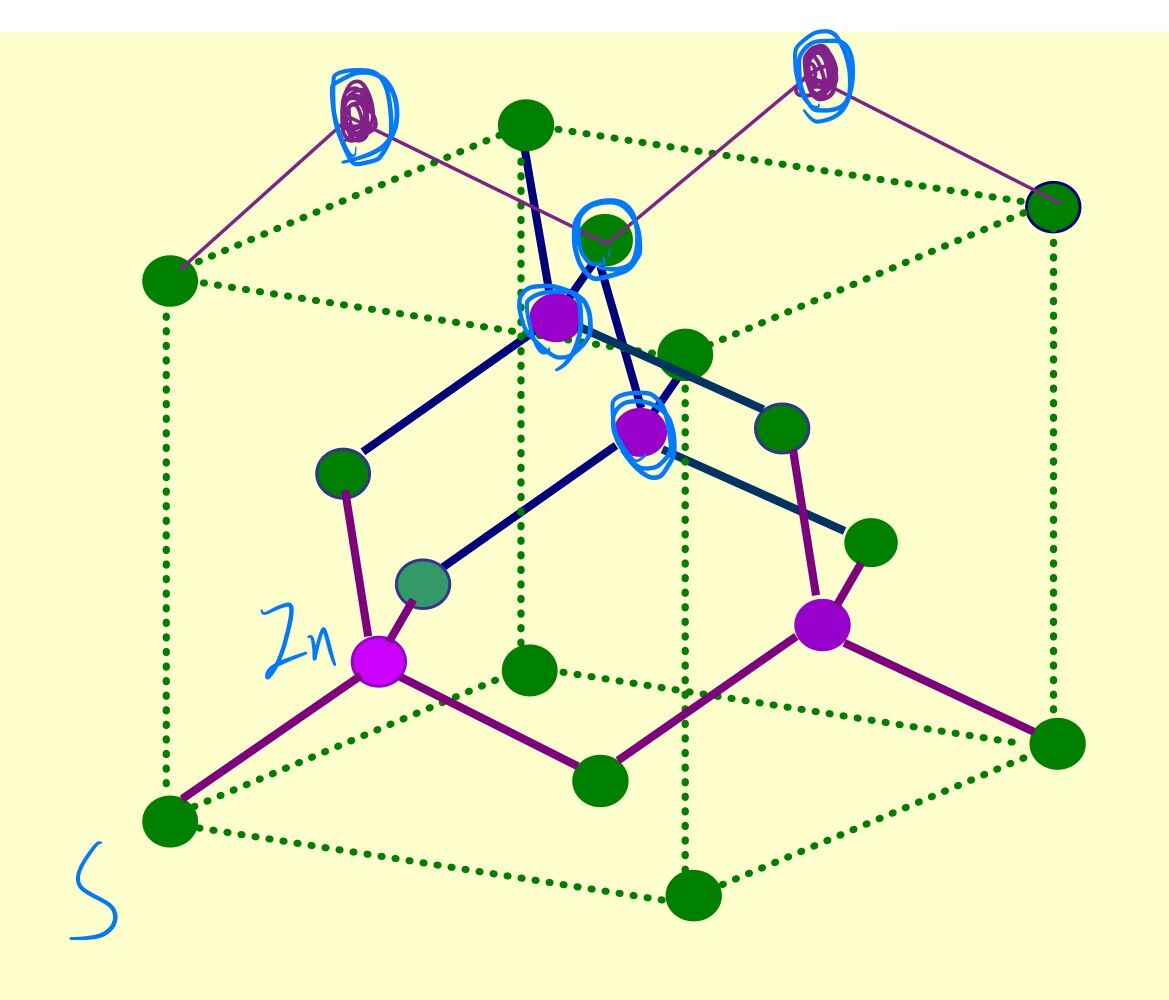
\includegraphics[scale=0.15]{基元}}
		\subfigure[等效面心立方晶格]{	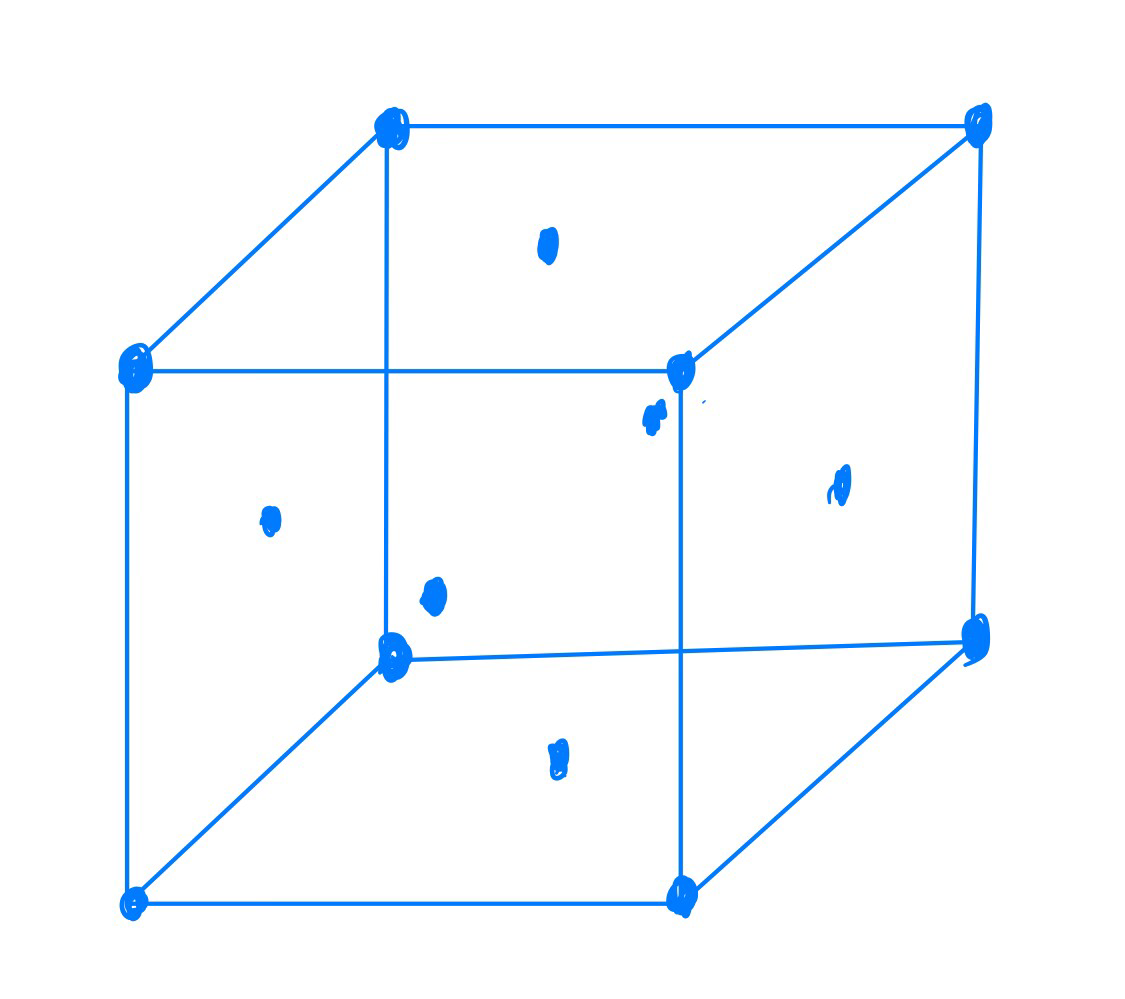
\includegraphics[scale=0.15]{面心}}
		\captionsetup{font={small},labelfont=bf}
		\caption{\heiti\zihao{-5}基元选取}
		
	\end{figure}
	
	
	闪锌矿的原胞如图3,连接顶点S原子到两个邻近的面心得到原胞基矢。
	\begin{figure}[!h]
		
		\centering
		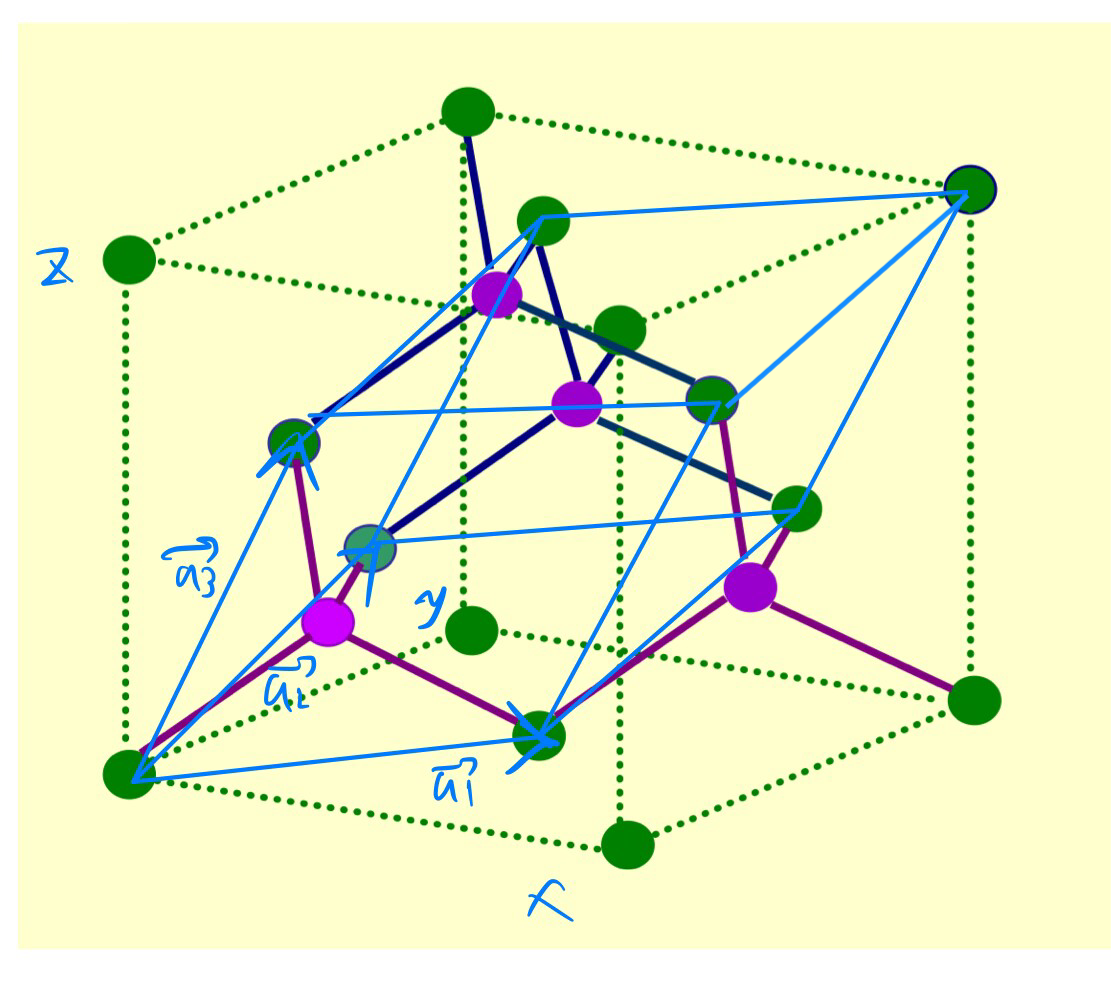
\includegraphics[scale=0.2]{原胞}
		\captionsetup{font={small},labelfont=bf}
		\caption{\heiti\zihao{-5}原胞}
		
	\end{figure}
	\begin{equation}
		\begin{cases}
			\vec{\alpha_1}=\frac{a}{2}\hat{x}+\frac{a}{2}\hat{y}\\
			\vec{\alpha_2}=\frac{a}{2}\hat{x}+\frac{a}{2}\hat{z}\\
			\vec{\alpha_3}=\frac{a}{2}\hat{y}+\frac{a}{2}\hat{z}
		\end{cases}
	\end{equation}
	
	
	可见在一个原胞中,内部包含了一个Zn原子,其余的三个Zn原子在原胞外,且原胞八个顶点的S原子各占有$ \frac{1}{8} $,共有一个Zn,一个S。对应闪锌矿的化学组成ZnS。其Wigner-Seitz原胞对应于体心立方的布里渊区,即为正菱形十二面体。
	
	
	\subsection{对称性}
	首先对面面心的连线为二重旋转轴,同时也为四重旋转反演轴,共3条;体对角线为三重旋转轴,共4条;同时晶格表面的面对角线,与该面面心与对面面心连线轴构成的平面均为反映面,共有6个反映面。由此得到闪锌矿的点群为$ T_d $点群。
	
	
	
	
	
	闪锌矿由不同原子构成,其失去了金刚石原有的四度螺旋轴。
	
	\subsection{倒易点阵与布里渊区}
	由于基元组成的晶格为面心立方,其倒易点阵为边长为$ \frac{4\pi}{a} $的体心立方。倒格子基矢
	\begin{equation}
		\begin{cases}
			\vec{b_1}=\frac{2\pi}{a}(\hat{x}+\hat{y}-\hat{z})\\
			\vec{b_2}=\frac{2\pi}{a}(\hat{x}-\hat{y}+\hat{z})\\
			\vec{b_3}=\frac{2\pi}{a}(-\hat{x}+\hat{y}+\hat{z})
		\end{cases}
	\end{equation}
	
	
	对应的第一布里渊区为一个截角八面体如图\ref{fig:4}
	\begin{figure}[!h]
		
		\centering
		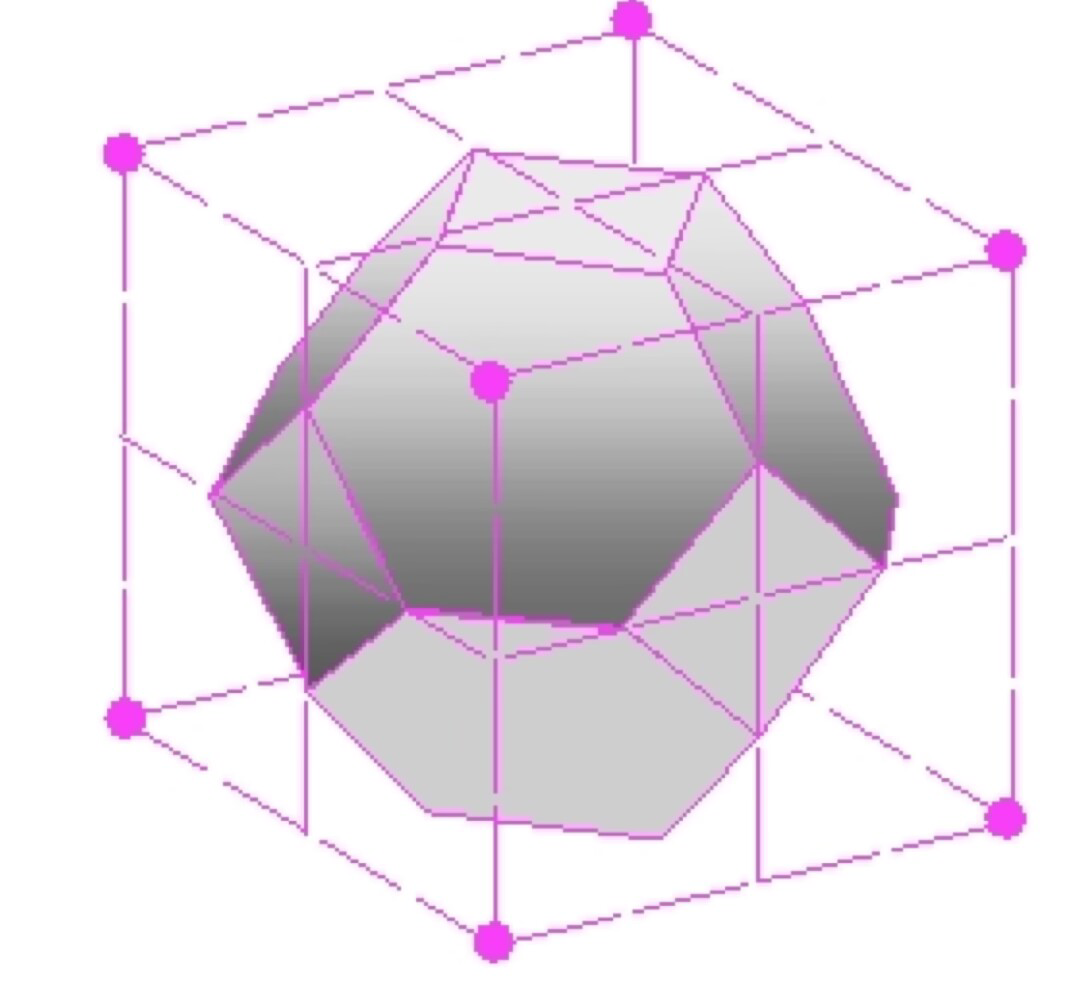
\includegraphics[scale=0.2]{布里渊区}
		\captionsetup{font={small},labelfont=bf}
		\caption{\heiti\zihao{-5}第一布里渊区}
		\label{fig:4}
	\end{figure}
	
	
	如图5进一步可以推知第二布里渊区为该体心立方本身(次近邻点为紫色,为近邻晶格的体心),第三布里渊区仍为截角八面体(第三近邻点为绿色,为对角晶格的体心)。
	\begin{figure}[!h]
		
		\centering
		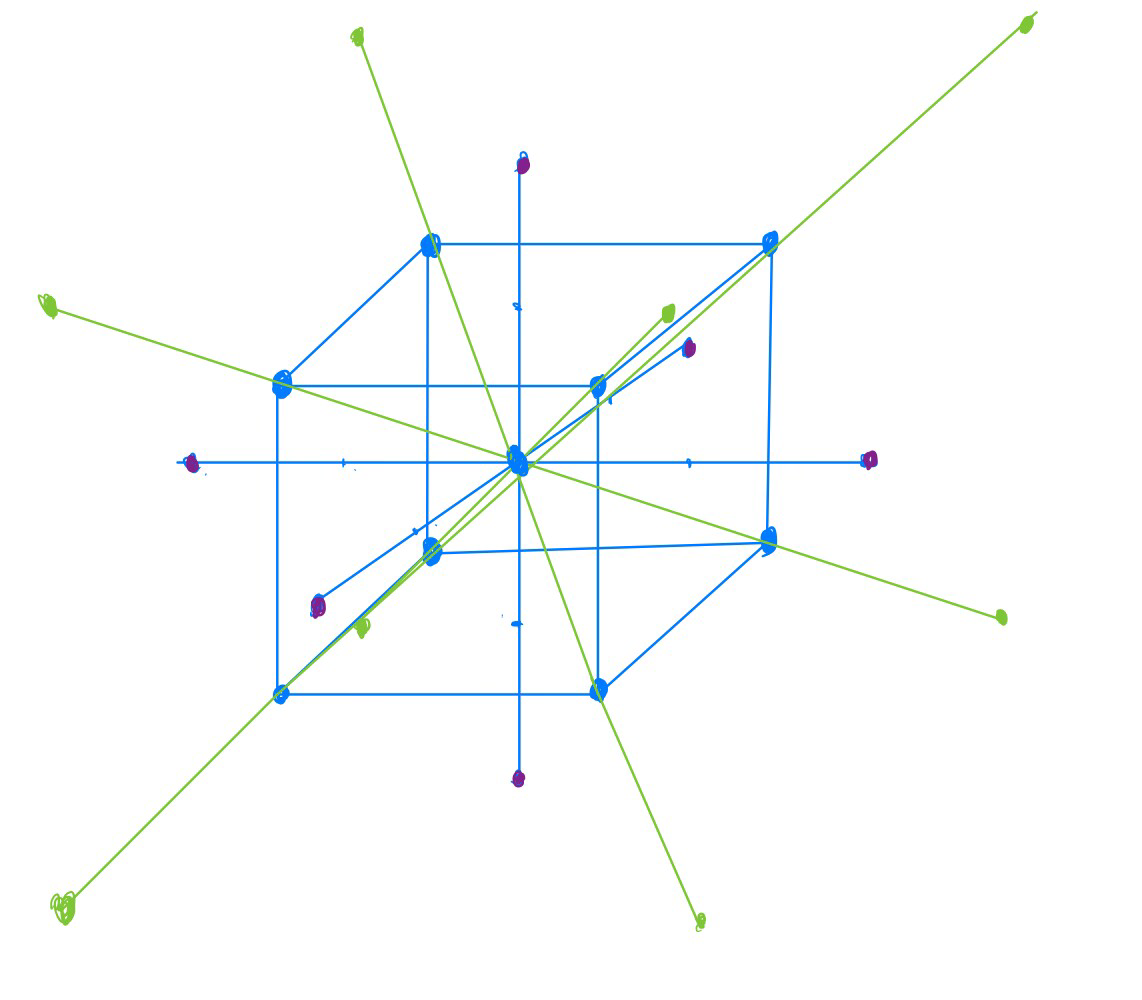
\includegraphics[scale=0.2]{高}
		\captionsetup{font={small},labelfont=bf}
		\caption{\heiti\zihao{-5}第2、3布里渊区}
		
	\end{figure}
\subsection{晶体衍射}
惯用晶胞中有8个原子,分别是4个S原子: $ 000,\ \frac{1}{2}\frac{1}{2}0,\ \frac{1}{2}0\frac{1}{2},\ 0\frac{1}{2}\frac{1}{2}  $和4个Zn原子:$ \frac{1}{4}\frac{1}{4}\frac{1}{4},\ \frac{3}{4}\frac{3}{4}\frac{1}{4},\ \frac{1}{4}\frac{3}{4}\frac{3}{4},\ \frac{3}{4}\frac{1}{4}\frac{3}{4}  $,令S原子的原子散射因子为$ f_a $,Zn原子的原子散射因子$ f_b $,对于波矢$ \boldmath{k}=\frac{2\pi}{a}(H,K,L) $,则闪锌矿的几何结构因子
\begin{equation}
	\begin{aligned}
		F_{HKL}&=f_a[1+\exp(i\pi(H+K))+\exp(i\pi(K+L))+\exp(i\pi(L+H))]\\
		&+f_b[\exp(i\frac{\pi}{2}(H+K+L))+\exp(i\frac{\pi}{2}(3H+3K+L))+\exp(i\frac{\pi}{2}(H+3K+3L))+\exp(i\frac{\pi}{2}(3H+K+3L))]\\
		&=(f_a+f_b\exp(i\frac{\pi}{2}(H+K+L)))[1+\exp(i\pi(H+K))+\exp(i\pi(K+L))+\exp(i\pi(L+H))]
	\end{aligned}
\label{eq:3}
\end{equation}
由此可见闪锌矿的几何结构因子类似于2个面心立方结构相差一定相位的线性组合。当H,K,L奇偶混杂时,$ F_{HKL}=0 $,衍射峰消失;当H,K,L全为奇数时,$ |F_{HKL}|=4\sqrt{f_a^2+f_b^2} $;当H,K,L全部是偶数,且H+K+L=4n(其中n为整数)时,达到极大值$ |F_{HKL}|=4(f_a+f_b) $。
\section{晶体结合}
ZnS通过共价键结合,每个Zn原子和S原子的配位数都是4,与金刚石类似,存在$ sp^3 $杂化。但是异类原子组成的晶体形成的共价键也包括离子键的成分。这里取8个惯用晶胞组成的大正方体,以该8个惯用晶胞共同的顶点为原点,在最接近的Zn与S原子的间距取为1的情况下,可得惯用晶胞正方体边长为$ a=\frac{4}{\sqrt{3}} $,可以计算ZnS的马德隆常数如下
\begin{equation}
	\alpha=\frac{4}{1}+\frac{4}{3}+12\sqrt{\frac{3}{11}}+12\sqrt{\frac{3}{19}}-12\frac{\sqrt{3}}{2\sqrt{2}}-\frac{6}{2}\frac{\sqrt{3}}{4}-\frac{24}{2}\frac{1}{2\sqrt{2}}-\frac{12}{4}\frac{\sqrt{3}}{4\sqrt{2}}-\frac{8}{8}\frac{1}{4}=2.3097
\end{equation}
该计算结果与标准结果1.638相比存在一定差距。如果进一步提高所取的晶格范围,可以得到更加接近的结果。
\section{晶格振荡}
分别使用l,m,n编号原子的
基矢$ \vec{a_1}=\frac{a}{2}(\hat{x}+\hat{z}),\vec{a_2}=\frac{a}{2}(\hat{x}+\hat{y}),\vec{a_3}=\frac{a}{2}(\hat{y}+\hat{z}) $方向序号。取S原子与临近沿对角线方向的一个Zn原子为原胞,S原子位于1位置,Zn原子位于2位置。偏移格点的位移用$ u^x,u^y,u^z $表示。


假设S与S原子间相互作用力系数为$ A $,Zn与Zn原子之间相互作用系数为$ B $,S与Zn之间的力相互作用系数为$ C $。S原子质量m,Zn原子质量为M。现在对第$ (l_1,m_1,n_1) $与$ (l_2,m_2,n_2) $的S原子和Zn原子作为原胞进行受力分析。


首先是S原子:
\begin{equation}
	\begin{aligned}
		m\ddot{u}^x_{l_1m_1n_1}&=-\frac{C}{3}(u^x_{l_1m_1n_1}+u^y_{l_1m_1n_1}+u^z_{l_1m_1n_1}-u^x_{l_2m_2n_2}-u^y_{l_2m_2n_2}-u^x_{l_2m_2n_2})\\
		&-\frac{C}{3}(u^x_{l_1m_1n_1}-u^x_{l_2(m_2-1)n_2}+u^y_{l_1m_1n_1}-u^y_{l_2(m_2-1)n_2}-u^z_{l_1m_1n_1}+u^z_{l_2(m_2-1)n_2})\\
		&-\frac{C}{3}(u^x_{l_1m_1n_1}-u^x_{l_2m_2(n_2-1)}-u^y_{l_1m_1n_1}+u^y_{l_2m_2(n_2-1)}-u^z_{l_1m_1n_1}+u^z_{l_2m_2(n_2-1)})\\
		&-\frac{C}{3}(u^x_{l_1m_1n_1}-u^x_{(l_2-1)m_2n_2}-u^y_{l_1m_1n_1}+u^y_{(l_2-1)m_2n_2}+u^z_{l_1m_1n_1}-u^z_{(l_2-1)m_2n_2})\\
		&+\frac{A}{2}\big[(u^x_{(l_1+1)m_1n_1}-u^x_{l_1m_1n_1})+(u^x_{(l_1-1)m_1n_1}-u^x_{l_1m_1n_1})+(u^x_{l_1(m_1+1)n_1}-u^x_{l_1m_1n_1})+(u^x_{l_1(m_1-1)n_1}-u^x_{l_1m_1n_1})\\
		&+(u^x_{(l_1+1)m_1(n_1-1)}-u^x_{l_1m_1n_1})+(u^x_{(l_1-1)m_1(n_1+1)}-u^x_{l_1m_1n_1})+(u^x_{l_1(m_1+1)(n_1-1)}-u^x_{l_1m_1n_1})+(u^x_{l_1(m_1-1)(n_1+1)}-u^x_{l_1m_1n_1})\\
		&+(u^y_{l_1(m_1+1)n_1}-u^y_{l_1m_1n_1})+(u^y_{l_1(m_1-1)n_1}-u^y_{l_1m_1n_1})-(u^y_{(l_1+1)m_1(n_1-1)}-u^y_{l_1m_1n_1})-(u^y_{(l_1-1)m_1(n_1+1)}-u^y_{l_1m_1n_1})\\
		&+(u^z_{(l_1+1)m_1n_1}-u^z_{l_1m_1n_1})+(u^z_{(l_1-1)m_1n_1}-u^z_{l_1m_1n_1})-(u^z_{l_1(m_1+1)(n_1-1)}-u^z_{l_1m_1n_1})-(u^z_{l_1(m_1-1)(n_1+1)}-u^z_{l_1m_1n_1})\big]\\
	\end{aligned}
\label{eq:5}
\end{equation}
\begin{equation}
	\begin{aligned}
		m\ddot{u}^y_{l_1m_1n_1}&=-\frac{C}{3}(u^x_{l_1m_1n_1}+u^y_{l_1m_1n_1}+u^z_{l_1m_1n_1}-u^x_{l_2m_2n_2}-u^y_{l_2m_2n_2}-u^x_{l_2m_2n_2})\\
		&-\frac{C}{3}(u^x_{l_1m_1n_1}-u^x_{l_2(m_2-1)n_2}+u^y_{l_1m_1n_1}-u^y_{l_2(m_2-1)n_2}-u^z_{l_1m_1n_1}+u^z_{l_2(m_2-1)n_2})\\
		&+\frac{C}{3}(u^x_{l_1m_1n_1}-u^x_{l_2m_2(n_2-1)}-u^y_{l_1m_1n_1}+u^y_{l_2m_2(n_2-1)}-u^z_{l_1m_1n_1}+u^z_{l_2m_2(n_2-1)})\\
		&+\frac{C}{3}(u^x_{l_1m_1n_1}-u^x_{(l_2-1)m_2n_2}-u^y_{l_1m_1n_1}+u^y_{(l_2-1)m_2n_2}+u^z_{l_1m_1n_1}-u^z_{(l_2-1)m_2n_2})\\
		&+\frac{A}{2}\big[(u^y_{l_1m_1(n_1+1)}-u^y_{l_1m_1n_1})+(u^y_{l_1m_1(n_1-1)}-u^y_{l_1m_1n_1})+(u^y_{l_1(m_1+1)n_1}-u^y_{l_1m_1n_1})+(u^y_{l_1(m_1-1)n_1}-u^y_{l_1m_1n_1})\\
		&+(u^y_{(l_1+1)m_1(n_1-1)}-u^y_{l_1m_1n_1})+(u^y_{(l_1-1)m_1(n_1+1)}-u^y_{l_1m_1n_1})+(u^y_{(l_1-1)(m_1+1)n_1}-u^y_{l_1m_1n_1})+(u^y_{(l_1+1)(m_1-1)n_1}-u^y_{l_1m_1n_1})\\
		&+(u^x_{l_1(m_1+1)n_1}-u^x_{l_1m_1n_1})+(u^x_{l_1(m_1-1)n_1}-u^x_{l_1m_1n_1})-(u^x_{(l_1+1)m_1(n_1-1)}-u^x_{l_1m_1n_1})-(u^x_{(l_1-1)m_1(n_1+1)}-u^x_{l_1m_1n_1})\\
		&+(u^z_{l_1m_1(n_1+1)}-u^z_{l_1m_1n_1})+(u^z_{l_1m_1(n_1-1)}-u^z_{l_1m_1n_1})-(u^z_{(l_1-1)(m_1+1)n_1}-u^z_{l_1m_1n_1})-(u^z_{(l_1+1)(m_1-1)n_1}-u^z_{l_1m_1n_1})\big]\\
	\end{aligned}
\end{equation}
\begin{equation}
	\begin{aligned}
		m\ddot{u}^z_{l_1m_1n_1}&=-\frac{C}{3}(u^x_{l_1m_1n_1}+u^y_{l_1m_1n_1}+u^z_{l_1m_1n_1}-u^x_{l_2m_2n_2}-u^y_{l_2m_2n_2}-u^x_{l_2m_2n_2})\\
		&+\frac{C}{3}(u^x_{l_1m_1n_1}-u^x_{l_2(m_2-1)n_2}+u^y_{l_1m_1n_1}-u^y_{l_2(m_2-1)n_2}-u^z_{l_1m_1n_1}+u^z_{l_2(m_2-1)n_2})\\
		&+\frac{C}{3}(u^x_{l_1m_1n_1}-u^x_{l_2m_2(n_2-1)}-u^y_{l_1m_1n_1}+u^y_{l_2m_2(n_2-1)}-u^z_{l_1m_1n_1}+u^z_{l_2m_2(n_2-1)})\\
		&-\frac{C}{3}(u^x_{l_1m_1n_1}-u^x_{(l_2-1)m_2n_2}-u^y_{l_1m_1n_1}+u^y_{(l_2-1)m_2n_2}+u^z_{l_1m_1n_1}-u^z_{(l_2-1)m_2n_2})\\
		&+\frac{A}{2}\big[(u^z_{l_1m_1(n_1+1)}-u^z_{l_1m_1n_1})+(u^z_{l_1m_1(n_1-1)}-u^z_{l_1m_1n_1})+(u^z_{(l_1+1)m_1n_1}-u^z_{l_1m_1n_1})+(u^z_{(l_1-1)m_1n_1}-u^y_{l_1m_1n_1})\\
		&+(u^z_{l_1(m_1+1)(n_1-1)}-u^z_{l_1m_1n_1})+(u^z_{l_1(m_1-1)(n_1+1)}-u^z_{l_1m_1n_1})+(u^z_{(l_1-1)(m_1+1)n_1}-u^z_{l_1m_1n_1})+(u^z_{(l_1+1)(m_1-1)n_1}-u^z_{l_1m_1n_1})\\
		&+(u^x_{(l_1+1)m_1n_1}-u^x_{l_1m_1n_1})+(u^x_{(l_1-1)m_1n_1}-u^x_{l_1m_1n_1})-(u^x_{l_1(m_1-1)(n_1+1)}-u^x_{l_1m_1n_1})-(u^x_{l_1(m_1+1)(n_1-1)}-u^x_{l_1m_1n_1})\\
		&+(u^y_{l_1m_1(n_1+1)}-u^y_{l_1m_1n_1})+(u^y_{l_1m_1(n_1-1)}-u^y_{l_1m_1n_1})-(u^y_{(l_1-1)(m_1+1)n_1}-u^y_{l_1m_1n_1})-(u^y_{(l_1+1)(m_1-1)n_1}-u^y_{l_1m_1n_1})\big]\\
	\end{aligned}
\end{equation}


类似对于Zn原子受力分析
\begin{equation}
	\begin{aligned}
		M\ddot{u}^x_{l_2m_2n_2}&=-\frac{C}{3}(u^x_{l_2m_2n_2}+u^y_{l_2m_2n_2}+u^z_{l_2m_2n_2}-u^x_{l_1m_1n_1}-u^y_{l_1m_1n_1}-u^x_{l_1m_1n_1})\\
		&-\frac{C}{3}(u^x_{l_2m_2n_2}-u^x_{l_1(m_1+1)n_1}+u^y_{l_2m_2n_2}-u^y_{l_1(m_1+1)n_2}-u^z_{l_2m_2n_2}+u^z_{l_1(m_1+1)n_1})\\
		&-\frac{C}{3}(u^x_{l_2m_2n_2}-u^x_{l_1m_1(n_1+1)}-u^y_{l_2m_2n_2}+u^y_{l_1m_1(n_1+1)}-u^z_{l_2m_2n_2}+u^z_{l_1m_1(n_1+1)})\\
		&-\frac{C}{3}(u^x_{l_2m_2n_2}-u^x_{(l_1+1)m_1n_1}-u^y_{l_2m_2n_2}+u^y_{(l_1+1)m_1n_1}+u^z_{l_2m_2n_2}-u^z_{(l_1+1)m_1n_1})\\
		&+\frac{B}{2}\big[(u^x_{(l_2+1)m_2n_2}-u^x_{l_2m_2n_2})+(u^x_{(l_2-1)m_2n_2}-u^x_{l_2m_2n_2})+(u^x_{l_2(m_2+1)n_2}-u^x_{l_2m_2n_2})+(u^x_{l_2(m_2-1)n_2}-u^x_{l_2m_2n_2})\\
		&+(u^x_{(l_2+1)m_2(n_2-1)}-u^x_{l_2m_2n_2})+(u^x_{(l_2-1)m_2(n_2+1)}-u^x_{l_2m_2n_2})+(u^x_{l_2(m_2+1)(n_2-1)}-u^x_{l_2m_2n_2})+(u^x_{l_2(m_2-1)(n_2+1)}-u^x_{l_2m_2n_2})\\
		&+(u^y_{l_2(m_2+1)n_2}-u^y_{l_2m_2n_2})+(u^y_{l_2(m_2-1)n_2}-u^y_{l_2m_2n_2})-(u^y_{(l_2+1)m_2(n_2-1)}-u^y_{l_2m_2n_2})-(u^y_{(l_2-1)m_2(n_2+1)}-u^y_{l_2m_2n_2})\\
		&+(u^z_{(l_2+1)m_2n_2}-u^z_{l_2m_2n_2})+(u^z_{(l_2-1)m_2n_2}-u^z_{l_2m_2n_2})-(u^z_{l_2(m_2+1)(n_2-1)}-u^z_{l_2m_2n_2})-(u^z_{l_2(m_2-1)(n_2+1)}-u^z_{l_2m_2n_2})\big]\\
	\end{aligned}
\end{equation}
\begin{equation}
	\begin{aligned}
		M\ddot{u}^y_{l_2,m_2,n_2}&=-\frac{C}{3}(u^x_{l_2m_2n_2}+u^y_{l_2m_2n_2}+u^z_{l_2m_2n_2}-u^x_{l_1m_1n_1}-u^y_{l_1m_1n_1}-u^x_{l_1m_1n_1})\\
		&-\frac{C}{3}(u^x_{l_2m_2n_2}-u^x_{l_1(m_1+1)n_1}+u^y_{l_2m_2n_2}-u^y_{l_1(m_1+1)n_2}-u^z_{l_2m_2n_2}+u^z_{l_1(m_1+1)n_1})\\
		&+\frac{C}{3}(u^x_{l_2m_2n_2}-u^x_{l_1m_1(n_1+1)}-u^y_{l_2m_2n_2}+u^y_{l_1m_1(n_1+1)}-u^z_{l_2m_2n_2}+u^z_{l_1m_1(n_1+1)})\\
		&+\frac{C}{3}(u^x_{l_2m_2n_2}-u^x_{(l_1+1)m_1n_1}-u^y_{l_2m_2n_2}+u^y_{(l_1+1)m_1n_1}+u^z_{l_2m_2n_2}-u^z_{(l_1+1)m_1n_1})\\
		&+\frac{B}{2}\big[(u^y_{l_2m_2(n_2+1)}-u^y_{l_2m_2n_2})+(u^y_{l_2m_2(n_2-1)}-u^y_{l_2m_2n_2})+(u^y_{l_2(m_2+1)n_2}-u^y_{l_2m_2n_2})+(u^y_{l_2(m_2-1)n_2}-u^y_{l_2m_2n_2})\\
		&+(u^y_{(l_2+1)m_2(n_2-1)}-u^y_{l_2m_2n_2})+(u^y_{(l_2-1)m_2(n_2+1)}-u^y_{l_2m_2n_2})+(u^y_{(l_2-1)(m_2+1)n_2}-u^y_{l_2m_2n_2})+(u^y_{(l_2+1)(m_2-1)n_2}-u^y_{l_2m_2n_2})\\
		&+(u^x_{l_2(m_2+1)n_2}-u^x_{l_2m_2n_2})+(u^x_{l_2(m_2-1)n_2}-u^x_{l_2m_2n_2})-(u^x_{(l_2+1)m_2(n_2-1)}-u^x_{l_2m_2n_2})-(u^x_{(l_2-1)m_2(n_2+1)}-u^x_{l_2m_2n_2})\\
		&+(u^z_{l_2m_2(n_2+1)}-u^z_{l_2m_2n_2})+(u^z_{l_2m_2(n_2-1)}-u^z_{l_2m_2n_2})-(u^z_{(l_2-1)(m_2+1)n_2}-u^z_{l_2m_2n_2})-(u^z_{(l_2+1)(m_2-1)n_2}-u^z_{l_2m_2n_2})\big]\\
	\end{aligned}
\end{equation}
\begin{equation}
	\begin{aligned}
		M\ddot{u}^z_{l_2,m_2,n_2}&=-\frac{C}{3}(u^x_{l_2m_2n_2}+u^y_{l_2m_2n_2}+u^z_{l_2m_2n_2}-u^x_{l_1m_1n_1}-u^y_{l_1m_1n_1}-u^x_{l_1m_1n_1})\\
		&+\frac{C}{3}(u^x_{l_2m_2n_2}-u^x_{l_1(m_1+1)n_1}+u^y_{l_2m_2n_2}-u^y_{l_1(m_1+1)n_2}-u^z_{l_2m_2n_2}+u^z_{l_1(m_1+1)n_1})\\
		&+\frac{C}{3}(u^x_{l_2m_2n_2}-u^x_{l_1m_1(n_1+1)}-u^y_{l_2m_2n_2}+u^y_{l_1m_1(n_1+1)}-u^z_{l_2m_2n_2}+u^z_{l_1m_1(n_1+1)})\\
		&-\frac{C}{3}(u^x_{l_2m_2n_2}-u^x_{(l_1+1)m_1n_1}-u^y_{l_2m_2n_2}+u^y_{(l_1+1)m_1n_1}+u^z_{l_2m_2n_2}-u^z_{(l_1+1)m_1n_1})\\
		&+\frac{B}{2}\big[(u^z_{l_2m_2(n_2+1)}-u^z_{l_2m_2n_2})+(u^z_{l_2m_2(n_2-1)}-u^z_{l_2m_2n_2})+(u^z_{(l_2+1)m_2n_2}-u^z_{l_2m_2n_2})+(u^z_{(l_2-1)m_2n_2}-u^y_{l_2m_2n_2})\\
		&+(u^z_{l_2(m_2+1)(n_2-1)}-u^z_{l_2m_2n_2})+(u^z_{l_2(m_2-1)(n_2+1)}-u^z_{l_2m_2n_2})+(u^z_{(l_2-1)(m_2+1)n_2}-u^z_{l_2m_2n_2})+(u^z_{(l_2+1)(m_2-1)n_2}-u^z_{l_2m_2n_2})\\
		&+(u^x_{(l_2+1)m_2n_2}-u^x_{l_2m_2n_2})+(u^x_{(l_2-1)m_2n_2}-u^x_{l_2m_2n_2})-(u^x_{l_2(m_2-1)(n_2+1)}-u^x_{l_2m_2n_2})-(u^x_{l_2(m_2+1)(n_2-1)}-u^x_{l_2m_2n_2})\\
		&+(u^y_{l_2m_2(n_2+1)}-u^y_{l_2m_2n_2})+(u^y_{l_2m_2(n_2-1)}-u^y_{l_2m_2n_2})-(u^y_{(l_2-1)(m_2+1)n_2}-u^y_{l_2m_2n_2})-(u^y_{(l_2+1)(m_2-1)n_2}-u^y_{l_2m_2n_2})\big]\\
	\end{aligned}
\label{eq:10}
\end{equation}


可以得到方程解的形式
\begin{equation}
	\boldsymbol{u}_{l_1m_1n_1}=\vec{S}\exp\big[i(\omega t-k_xa\frac{l_1+m_1}{2}-k_ya\frac{m_1+n_1}{2}-k_za\frac{l_1+n_1}{2})\big]
\end{equation}
\begin{equation}
	\boldsymbol{u}_{l_2m_2n_2}=\vec{Z}\exp\big[i(\omega t-k_xa\frac{l_2+m_2}{2}-k_ya\frac{m_2+n_2}{2}-k_za\frac{l_2+n_2}{2})\big]
\end{equation}
根据S原子和Zn原子位置关系,$ (l_2,m_2,n_2)=(l_1+\frac{1}{4},m_1+\frac{1}{4},n_1+\frac{1}{4}) $
\begin{equation}
	\boldsymbol{u}_{l_2m_2n_2}=\vec{Z}\exp\big[i(\omega t-k_xa\frac{l_1+m_1+\frac{1}{2}}{2}-k_ya\frac{m_1+n_1+\frac{1}{2}}{2}-k_za\frac{l_1+n_1+\frac{1}{2}}{2})\big]
\end{equation}
将解反带回方程(\ref{eq:5})-(\ref{eq:10}),为便于计算,这里取$ \boldsymbol{k}=(k,0,0) $即波矢沿x方向,可以得到以下线性方程组
\begin{equation}
	\big\{m\omega^2-\frac{4}{3}C+A[4\cos(\frac{k}{2}a)-4]\big\}S_x+\frac{4}{3}C\cos(\frac{k}{4}a)Z_x=0
\end{equation}
\begin{equation}
	\big\{m\omega^2-\frac{4}{3}C+A[2\cos(\frac{k}{2}a)-2]\big\}S_y+\frac{4}{3}C\cos(\frac{k}{4}a)Z_y-i\frac{4}{3}C\sin(\frac{k}{4}a)Z_z=0
\end{equation}
\begin{equation}
	\big\{m\omega^2-\frac{4}{3}C+A[2\cos(\frac{k}{2}a)-2]\big\}S_z+\frac{4}{3}C\cos(\frac{k}{4}a)Z_z-i\frac{4}{3}C\sin(\frac{k}{4}a)Z_y=0
\end{equation}
\begin{equation}
	\big\{M\omega^2-\frac{4}{3}C+B[4\cos(\frac{k}{2}a)-4]\big\}Z_x+\frac{4}{3}C\cos(\frac{k}{4}a)S_x=0
\end{equation}
\begin{equation}
	\big\{M\omega^2-\frac{4}{3}C+B[2\cos(\frac{k}{2}a)-2]\big\}Z_y+\frac{4}{3}C\cos(\frac{k}{4}a)S_y+i\frac{4}{3}C\sin(\frac{k}{4}a)S_z=0
\end{equation}
\begin{equation}
	\big\{M\omega^2-\frac{4}{3}C+B[2\cos(\frac{k}{2}a)-2]\big\}Z_z+\frac{4}{3}C\cos(\frac{k}{4}a)S_z+i\frac{4}{3}C\sin(\frac{k}{4}a)S_y=0
\end{equation}


带入Mathematica进行求解行列式得到色散关系,根据有解条件,得到符合物理实际的6个正根
\begin{figure}[!h]
	\centering
	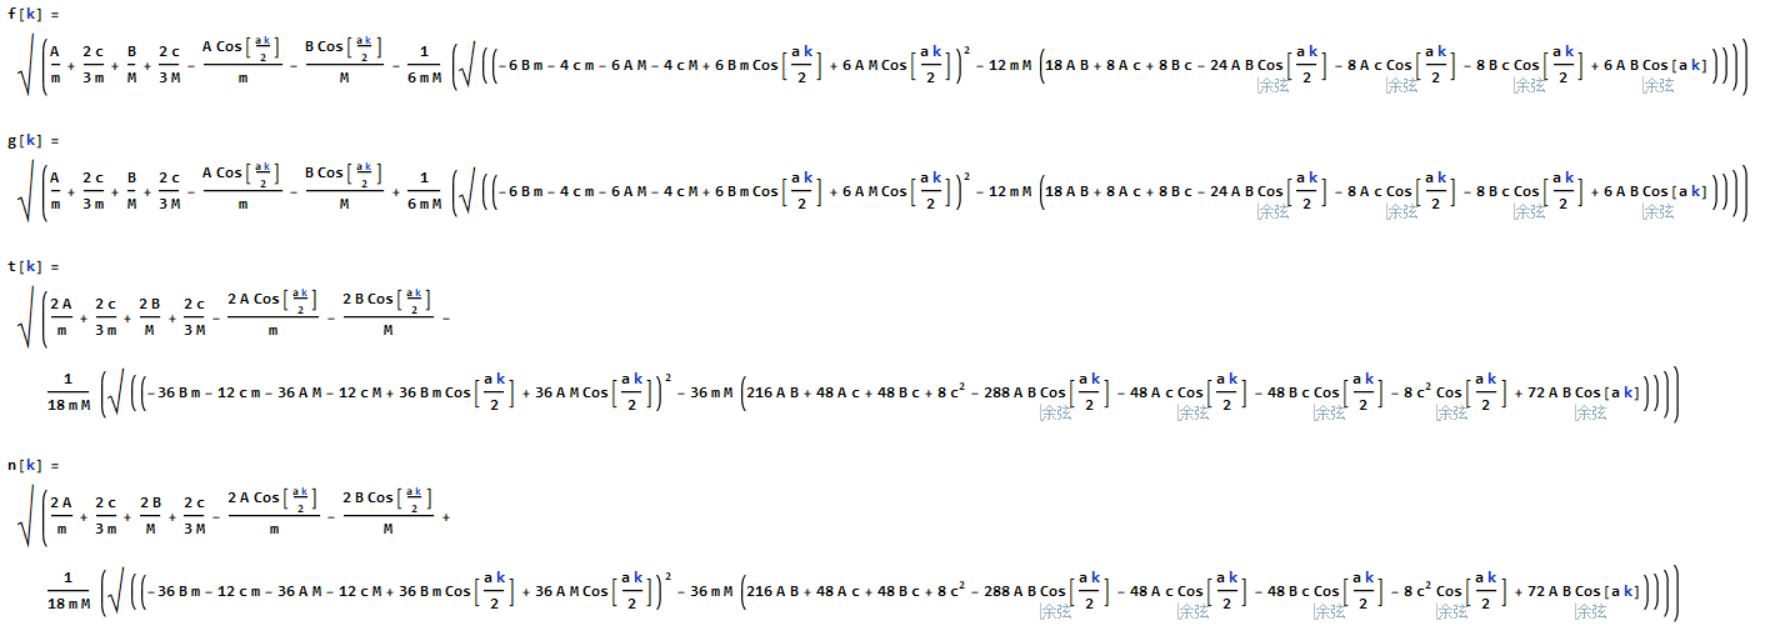
\includegraphics[scale=0.53]{w}
	\captionsetup{font={small},labelfont=bf}
\end{figure}
其中f[k],t[k]对应声学支,$ k\rightarrow0 $时$ \omega\rightarrow0 $;g[k],n[k]对应光学支,$ k\rightarrow0 $时$ \omega\rightarrow\sqrt{\frac{4C}{3}(\frac{1}{m}+\frac{1}{M})} $;f[k],g[k]均为二重根,t[k],n[k]为单根


带入$ \frac{M}{m}=\frac{65}{32} $,并假设$ A=B=C $,可得如图\ref{fig:6}色散关系
	\begin{figure}[!h]
	\centering
	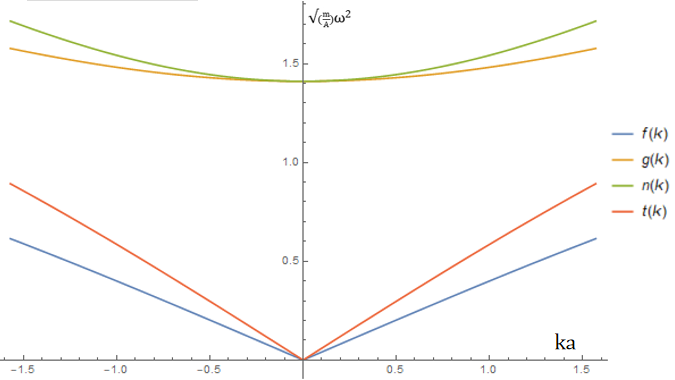
\includegraphics[scale=1]{vib}
	\captionsetup{font={small},labelfont=bf}
	\caption{\heiti\zihao{-5}ZnS晶体色散关系}
	\label{fig:6}%label加最后才可以引用正常
\end{figure}

\section{晶体能带}
\subsection{近自由电子近似}
根据图\ref{fig:4},可见由于能隙是Bloch波入射与反射波的干涉结果,根据式(\ref{eq:3})得到的几何结构因子,可知在第一布里渊区的$ (\pm1,0,0),(0,\pm1,0),(0,0,\pm1) $的三个方向上$ F_{HKL} =0$,界面上的能隙为0 。因此得到简约布里渊区能带如图\ref{fig:7},可得第1、2布里渊区边界不存在禁带。
	\begin{figure}[!h]
	\centering
	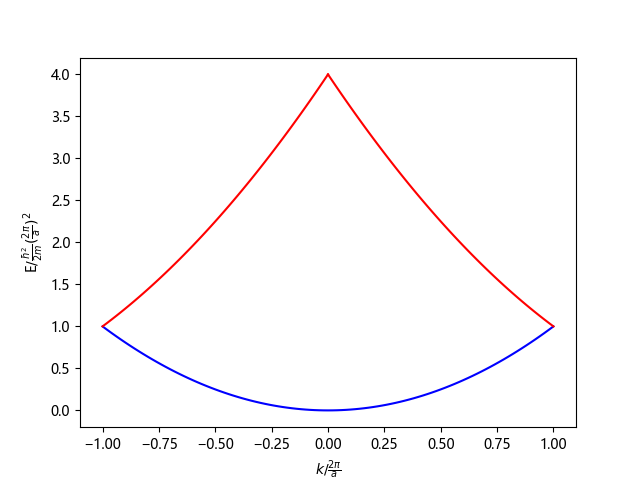
\includegraphics[scale=1]{freeband}
	\captionsetup{font={small},labelfont=bf}
	\caption{\heiti\zihao{-5}近自由电子近似下ZnS简约能带}
	\label{fig:7}%label加最后才可以引用正常
\end{figure}

\subsection{紧束缚近似}
考虑ZnS结构的S带,得到方程为
\begin{equation}
	\alpha\big[(\epsilon_A-E)-\sum_{\vec{R}_l}J_A(\vec{R}_S)\exp(-i\vec{k}\cdot\vec{R}_S)\big]-\beta\sum_{\vec{R}_l}J_{AB}(\vec{R}_S)\exp(i\vec{k}\cdot(\vec{R}_l+\vec{r}_A-\vec{r}_B))=0
\end{equation}
\begin{equation}
	\alpha\sum_{\vec{R}_l}J_{BA}(\vec{R}_S)\exp(i\vec{k}\cdot(\vec{R}_l-\vec{r}_A+\vec{r}_B))-\beta\big[(\epsilon_B-E)-\sum_{\vec{R}_l}J_B(\vec{R}_S)\exp(-i\vec{k}\cdot\vec{R}_S)\big]=0
\end{equation}
其中A对应Zn原子,B对应S原子,其中
\begin{equation}
	J_A=-\int\phi_A^*(\vec{\xi}-\vec{R}_S-\vec{r}_A)\big[V(\vec{\xi})-U_A(\vec{\xi}-\vec{r}_A)\big]\phi_A(\vec{\xi}-\vec{r}_A)d\vec{\xi}
\end{equation}
\begin{equation}
	J_B=-\int\phi_B^*(\vec{\xi}-\vec{R}_S-\vec{r}_B)\big[V(\vec{\xi})-U_B(\vec{\xi}-\vec{r}_B)\big]\phi_B(\vec{\xi}-\vec{r}_B)d\vec{\xi}
\end{equation}
\begin{equation}
	J_{AB}=-\int\phi_A^*(\vec{\xi}-\vec{R}_S-\vec{r}_A)\big[V(\vec{\xi})-U_B(\vec{\xi}-\vec{r}_B)\big]\phi_B(\vec{\xi}-\vec{r}_B)d\vec{\xi}
\end{equation}
\begin{equation}
	J_{BA}=-\int\phi_B^*(\vec{\xi}-\vec{R}_S-\vec{r}_B)\big[V(\vec{\xi})-U_A(\vec{\xi}-\vec{r}_A)\big]\phi_A(\vec{\xi}-\vec{r}_A)d\vec{\xi}
\end{equation}


带入只考虑最邻近原子
\begin{equation}
	\left|
	\begin{matrix}
		\epsilon_A-E-J_A & -2J_{AB}\big[\exp(i\frac{k_za}{4})\cos(\frac{k_x-k_y}{4}a)+\exp(-i\frac{k_za}{4})\cos(\frac{k_x+k_y}{4}a)\big]\\
		-2J_{BA}\big[\exp(i\frac{k_za}{4})\cos(\frac{k_x+k_y}{4}a)+\exp(-i\frac{k_za}{4})\cos(\frac{k_x-k_y}{4}a)\big] & \epsilon_ B-E-J_B
	\end{matrix}
\right|=0
\end{equation}
假设$ J_{AB}=J_{BA} $,得到结果
\begin{equation}
	E_{\pm}(\vec{k})=\frac{\epsilon_A+\epsilon_B-J_A-J_B}{2} \pm \sqrt{(\frac{\epsilon_A-\epsilon_B-J_A+J_B}{2})^2+16J_{AB}^2(\cos^2\frac{k_xa}{4}\cos^2\frac{k_ya}{4}\cos^2\frac{k_za}{4}+\sin^2\frac{k_xa}{4}\sin^2\frac{k_ya}{4}\sin^2\frac{k_za}{4})}
\end{equation}
\subsection{空格子模型}
取波矢k沿[010]方向,根据面心立方结构,取k单位$ \frac{2\pi}{a} $,E单位$ \frac{\hbar^2}{2m}(\frac{2\pi}{a})^2 $,可得一下各情况


(1)($ n_xn_yn_z $)=(000)
\begin{equation}
	E_1=(k_y)^2
\end{equation}
能量范围$ 0\rightarrow 1 \times \frac{\hbar^2}{2m}(\frac{2\pi}{a})^2 $,非简并。


(2)($ n_xn_yn_z $)=(1$\bar{1}1$), (1$\bar{1}$$\bar{1}$), ($\bar{1}$$\bar{1}$1), ($\bar{1}$$\bar{1}$$\bar{1}$)
\begin{equation}
	E_2=\big[1+(k_y-1)^2+1\big]
\end{equation}
能量范围$ 3\rightarrow 2 \times \frac{\hbar^2}{2m}(\frac{2\pi}{a})^2 $,4重简并。


(3)($ n_xn_yn_z $)=(111), (11$\bar{1}$), ($\bar{1}$11), ($\bar{1}$1$\bar{1}$)
\begin{equation}
	E_3=\big[1+(k_y+1)^2+1\big]
\end{equation}
能量范围$ 3\rightarrow 6 \times \frac{\hbar^2}{2m}(\frac{2\pi}{a})^2 $,4重简并。


(4)($ n_xn_yn_z $)=(0$\bar{2}0$)
\begin{equation}
	E_4=(k_y-2)^2
\end{equation}
能量范围$ 4\rightarrow 1 \times \frac{\hbar^2}{2m}(\frac{2\pi}{a})^2 $,非简并。


(5)($ n_xn_yn_z $)=(200), ($\bar{2}$00), (00$\bar{2}$), (002)
\begin{equation}
	E_5=\big[(k_y+1)^2+4\big]
\end{equation}
能量范围$ 4\rightarrow 5 \times \frac{\hbar^2}{2m}(\frac{2\pi}{a})^2 $,4重简并。


(6)($ n_xn_yn_z $)=(020)
\begin{equation}
	E_6=(k_y+2)^2
\end{equation}
能量范围$ 4\rightarrow 9 \times \frac{\hbar^2}{2m}(\frac{2\pi}{a})^2 $,非简并。
	\begin{figure}[!h]
	\centering
	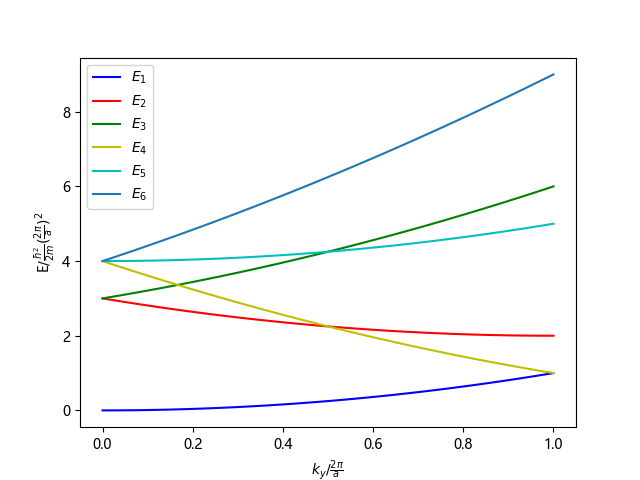
\includegraphics[scale=1]{empty}
	\captionsetup{font={small},labelfont=bf}
	\caption{\heiti\zihao{-5}空格子模型能带}
\end{figure}

\subsection{能态密度}
将紧束缚近似结果带入能态密度为
\begin{equation}
	\begin{aligned}
		N(E)&=\frac{1}{4\pi^3}\oiint_{E=Const}\dfrac{dS}{|\nabla_kE(k)|}\\
		&=\frac{\sqrt{(\frac{\epsilon_A-\epsilon_B-J_A+J_B}{2})^2+16J_{AB}^2(\cos^2\frac{k_xa}{4}\cos^2\frac{k_ya}{4}\cos^2\frac{k_za}{4}+\sin^2\frac{k_xa}{4}\sin^2\frac{k_ya}{4}\sin^2\frac{k_za}{4})}}{8\pi^3aJ_{AB}^2}\\
		&\oiint_{E=Const}\dfrac{dS}{\sqrt{\sin^2\frac{k_xa}{2}\cos^2\frac{k_y+k_z}{4}a\cos^2\frac{k_y-k_z}{4}a+\sin^2\frac{k_ya}{2}\cos^2\frac{k_x+k_z}{4}a\cos^2\frac{k_x-k_z}{4}a+\sin^2\frac{k_za}{2}\cos^2\frac{k_y+k_x}{4}a\cos^2\frac{k_y-k_x}{4}a}}
	\end{aligned}
\end{equation}
存在Van Hove奇点$ \boldsymbol{k}=\frac{2\pi}{a}(0,0,0),\ \frac{2\pi}{a}(1,0,0),\ \frac{2\pi}{a}(1,1,0),\ \frac{2\pi}{a}(1,1,1),\ \frac{2\pi}{a}(\frac{1}{2},\frac{1}{2},\frac{1}{2}) $

\section{晶体电子运动}


利用紧束缚近似结果,ZnS晶体中电子运动的速度
\begin{equation}
	\begin{aligned}
		\boldsymbol{v}&=\frac{1}{\hbar}\nabla_kE\\
		&=\frac{2aJ_{AB}^2(\hat{x}\sin\frac{k_xa}{2}\cos\frac{k_y+k_z}{4}a\cos\frac{k_y-k_z}{4}a + \hat{y}\sin\frac{k_ya}{2}\cos\frac{k_x+k_z}{4}a\cos\frac{k_x-k_z}{4}a + \hat{z}\sin\frac{k_za}{2}\cos\frac{k_y+k_x}{4}a\cos\frac{k_y-k_x}{4}a )} {\hbar \sqrt{(\frac{\epsilon_A-\epsilon_B-J_A+J_B}{2})^2+16J_{AB}^2(\cos^2\frac{k_xa}{4}\cos^2\frac{k_ya}{4}\cos^2\frac{k_za}{4}+\sin^2\frac{k_xa}{4}\sin^2\frac{k_ya}{4}\sin^2\frac{k_za}{4})}}
	\end{aligned}
\end{equation}
取k沿x方向,观察速度规律,可得速度也沿x方向,变化规律如图\ref{fig:9},速度在能带底和顶均为0,在中间处存在极大值。
\begin{equation}
	\boldsymbol{v}=\frac{2aJ_{AB}^2\sin\frac{k_xa}{2}} {\hbar \sqrt{(\frac{\epsilon_A-\epsilon_B-J_A+J_B}{2})^2+16J_{AB}^2\cos^2\frac{k_xa}{4}}}\hat{x}
\end{equation}
	\begin{figure}[!h]
	\centering
	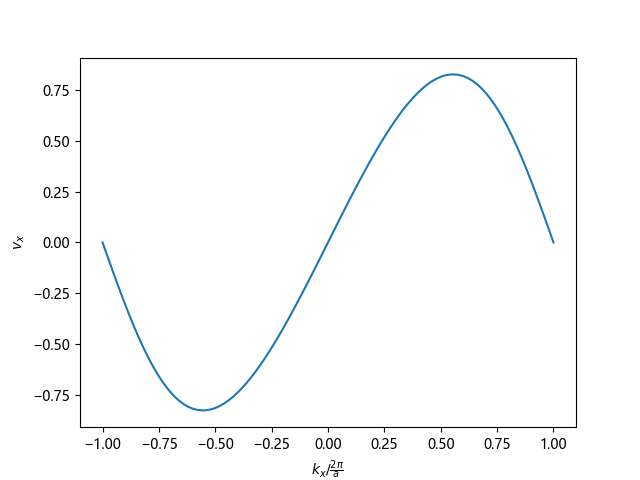
\includegraphics[scale=1]{v}
	\captionsetup{font={small},labelfont=bf}
	\caption{\heiti\zihao{-5}电子运动速度规律}
	\label{fig:9}
\end{figure}

进一步可以得到电子的有效质量矩阵
\begin{equation}
	\big[\frac{1}{m^*}\big]=\frac{1}{\hbar^2}
	\left[
	\begin{matrix}
		E_{xx}& E_{xy}& E_{xz}\\
		E_{yx}& E_{yy}& E_{yz}\\
		E_{zx}& E_{zy}& E_{zz}
	\end{matrix}\right]
\end{equation}
其中各矩阵元为
	\begin{figure}[!h]
	\centering
	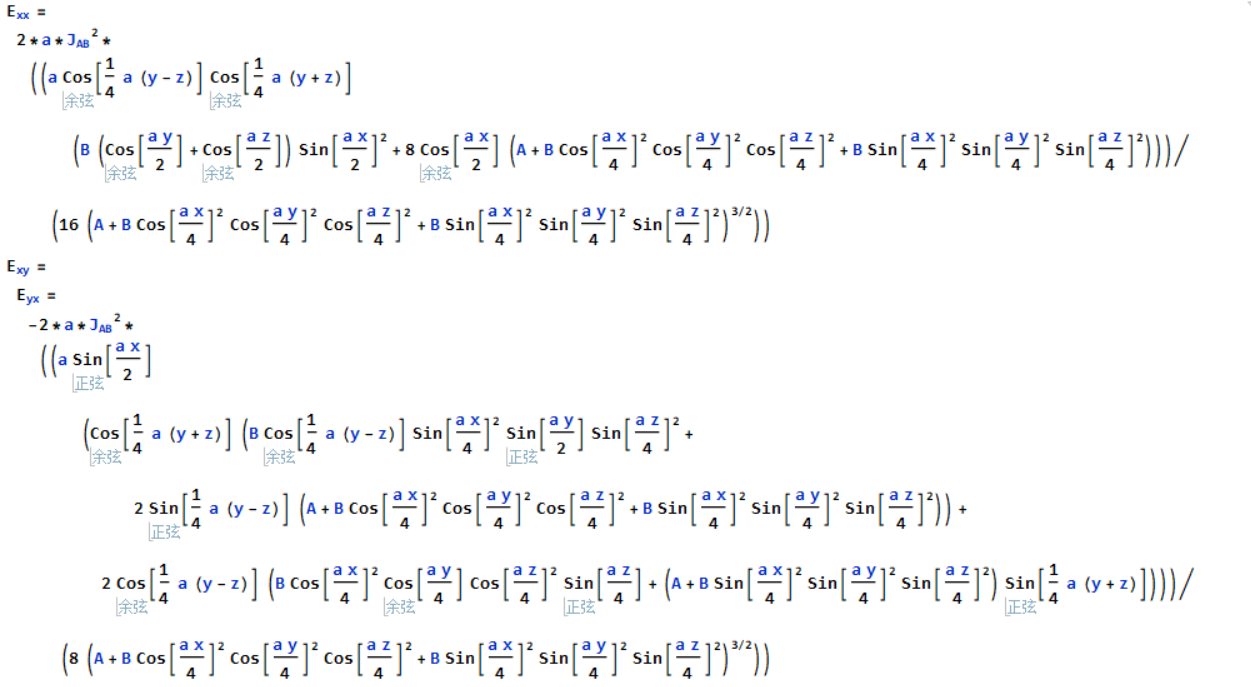
\includegraphics[scale=0.75]{m1}
	\captionsetup{font={small},labelfont=bf}
\end{figure}
	\begin{figure}[!h]
	\centering
	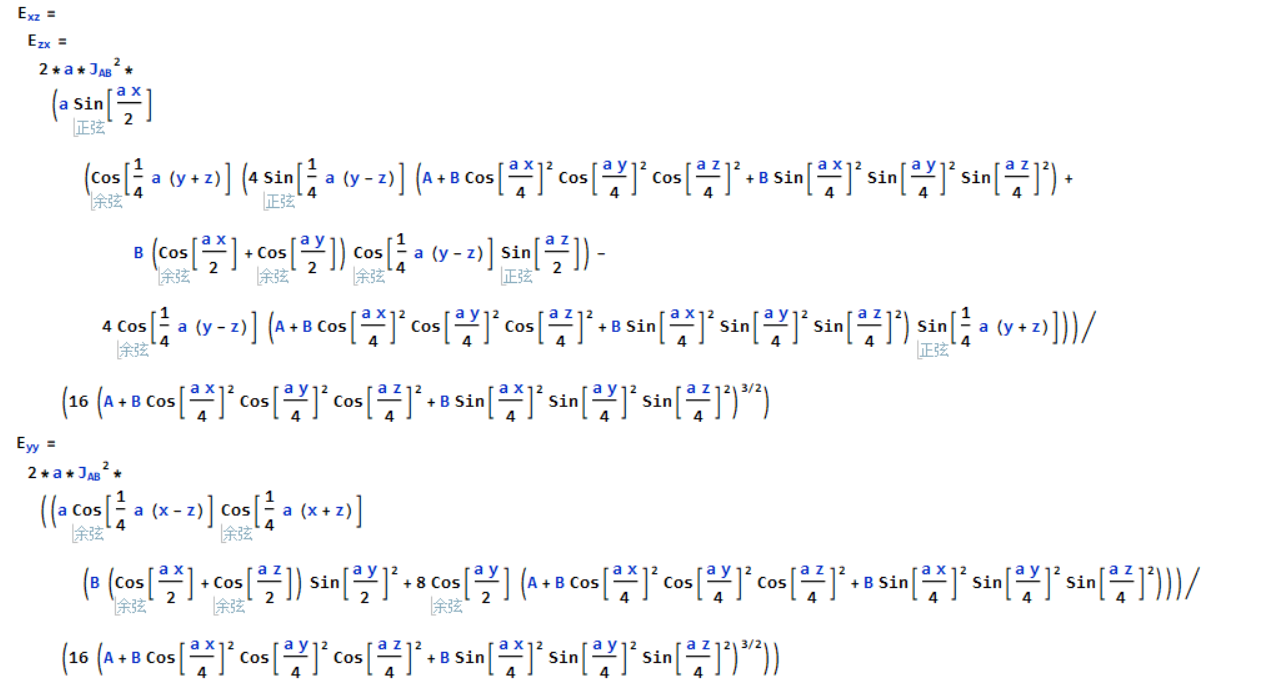
\includegraphics[scale=0.75]{m2}
	\captionsetup{font={small},labelfont=bf}
\end{figure}
	\begin{figure}[!h]
	\centering
	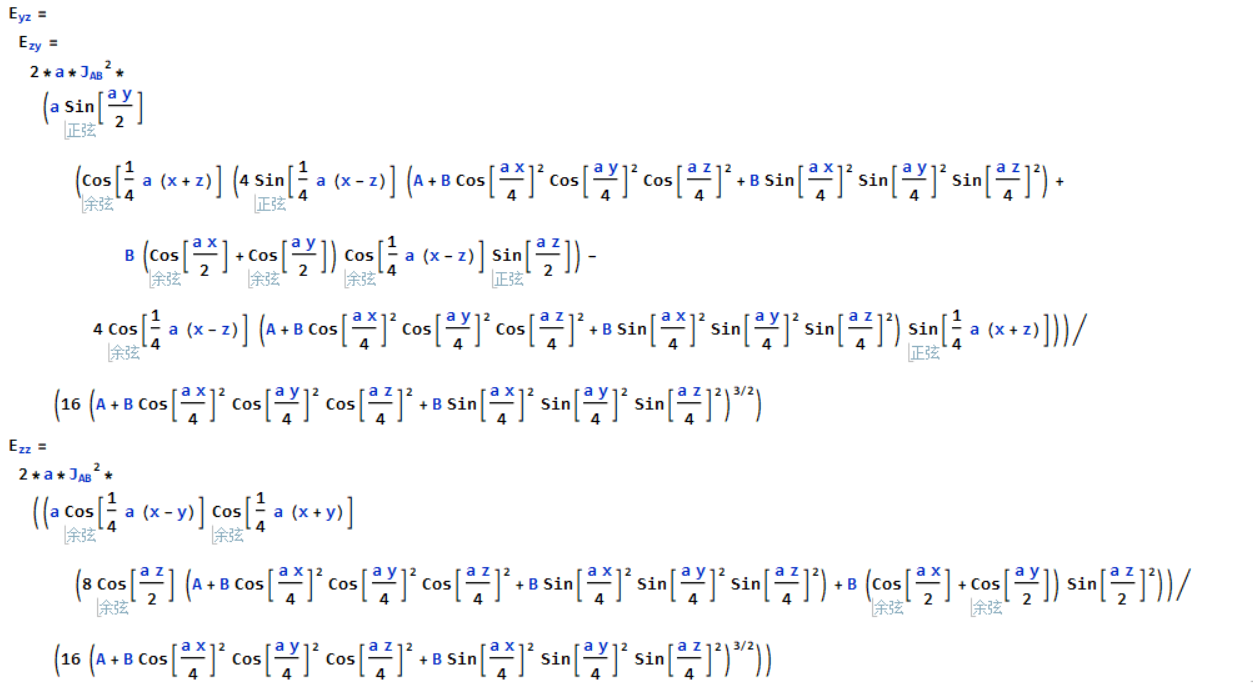
\includegraphics[scale=0.75]{m3}
	\captionsetup{font={small},labelfont=bf}
\end{figure}
其中$ A=(\frac{\epsilon_A-\epsilon_B-J_A+J_B}{2})^2 $, $ B=16J_{AB}^2 $,x,y,z分别代表$ k_x, k_y, k_y $


对于在加了外磁场的晶格中运动的电子,假设磁场沿z方向。分析在$ k_z=0 $的平面运动的电子,垂直于磁场方向的速度
\begin{equation}
	|v_{\perp}|=\frac{2aJ_{AB}^2\sqrt{\sin^2\frac{k_xa}{2}\cos^4\frac{k_ya}{4}+\sin^2\frac{k_ya}{2}\cos^4\frac{k_xa}{4}}} {\hbar \sqrt{(\frac{\epsilon_A-\epsilon_B-J_A+J_B}{2})^2+16J_{AB}^2\cos^2\frac{k_xa}{4}\cos^2\frac{k_ya}{4}}}
\end{equation}
可得电子回旋运动的周期
\begin{equation}
	T=\frac{\hbar^2}{2aJ_{AB}^2eB}\oint_{E=Const}\dfrac{ \sqrt{(\frac{\epsilon_A-\epsilon_B-J_A+J_B}{2})^2+16J_{AB}^2\cos^2\frac{k_xa}{4}\cos^2\frac{k_ya}{4}}} {\sqrt{\sin^2\frac{k_xa}{2}\cos^4\frac{k_ya}{4}+\sin^2\frac{k_ya}{2}\cos^4\frac{k_xa}{4}}}d\vec{k}
\end{equation}


在磁场中加入沿磁场的交变电场,发生回旋共振时,考虑处于能带底的电子$ \boldsymbol{k}=(000) $,此时有效质量退化为标量
\begin{equation}
	m^*=\hbar^2\frac{\sqrt{(\frac{\epsilon_A-\epsilon_B-J_A+J_B}{2})^2+16J_{AB}^2}}{a^2J_{AB}^2}
\end{equation}
可得共振频率
\begin{equation}
	\omega_c=\frac{eBa^2J_{AB}^2}{\hbar^2\sqrt{(\frac{\epsilon_A-\epsilon_B-J_A+J_B}{2})^2+16J_{AB}^2}}
\end{equation}

也可取能带顶$ k=(\frac{\pi}{a},\frac{\pi}{a},\frac{\pi}{a}) $,对角化可得主轴有效质量
\begin{equation}
	\begin{aligned}
		\begin{cases}
			&m_1=m_2=\frac{\hbar^2\sqrt{4(\frac{\epsilon_A-\epsilon_B-J_A+J_B}{2})^2+16J_{AB}^2}}{a^2J_{AB}^2}\\
			&m_3=-2\frac{\hbar^2\sqrt{4(\frac{\epsilon_A-\epsilon_B-J_A+J_B}{2})^2+16J_{AB}^2}}{a^2J_{AB}^2}
		\end{cases}
	\end{aligned}
\end{equation}
取$\theta$为磁场方向与主轴3的夹角
\begin{equation}
	m_c^*=\big(\frac{\sin^2\theta}{m_1m_3}+\frac{\cos^2\theta}{m_1^2}\big)^{-\frac{1}{2}}=\frac{\hbar^2\sqrt{4(\frac{\epsilon_A-\epsilon_B-J_A+J_B}{2})^2+16J_{AB}^2}}{a^2J_{AB}^2} \big(\frac{1+\cos^2\theta}{2}\big)^{-\frac{1}{2}}
\end{equation}
该点共振频率
\begin{equation}
	\omega_c=\frac{eBa^2J_{AB}^2}{\hbar^2\sqrt{4(\frac{\epsilon_A-\epsilon_B-J_A+J_B}{2})^2+16J_{AB}^2}}\big(\frac{1+\cos^2\theta}{2}\big)^{\frac{1}{2}}
\end{equation}


根据三维自由电子气模型,在磁场中能量随磁场变化周期
\begin{equation}
	\Delta(\frac{1}{B})=\frac{2\pi e}{\hbar A_F}=\frac{2e}{\hbar(3\pi^2n)^{\frac{2}{3}}}
\end{equation}
\end{document}